 \usetikzlibrary{calc} 
  \begin{tikzpicture}
    \node [anchor=south west] (img) at (0,0) {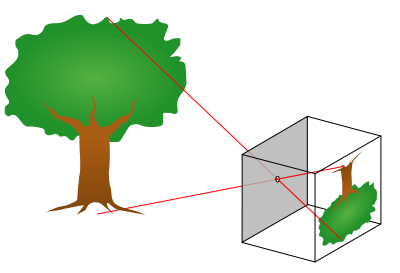
\includegraphics[width=\textwidth]{pinhole.png}};
    \begin{scope}[x={(img.south east)},y={(img.north west)}]
      \fill [yellow] (0.75,1.2) node (sun) {} ellipse (0.06 and 0.08);
\coordinate (tree) at (0.2,0.7);
      \foreach \y in {10, 20, 30} 
      {
        \draw [very thick,yellow] ($(sun) + (-150+\y:.1)$) -- ($(tree) + (80-2*\y:.3)$) node [inner sep=0] (trays) {};
	}
    \end{scope}
  \end{tikzpicture}
